\documentclass[11pt]{article}

\usepackage{algorithm2e}
\usepackage{algorithmic} 
\usepackage{amsmath}
\usepackage{amsthm}
\usepackage{booktabs}
\usepackage{dcolumn} 
\usepackage{epstopdf}
\usepackage{fourier}
\usepackage{fullpage}
\usepackage{graphicx}
\usepackage{hyperref}
\usepackage{longtable} 
\usepackage{natbib}
\usepackage{rotating}
\usepackage{tabularx}
\usepackage{tikz} 
\usepackage{xcolor} 

\hypersetup{
  colorlinks = TRUE,
  citecolor=blue,
  linkcolor=red,
  urlcolor=black
}

\DeclareMathOperator*{\argmax}{\arg\!\max}

\newcommand{\starlanguage}{Significance indicators: $p \le 0.05:*$,
  .$p \le 0.01:**$ and $p \le .001:***$.}  

\newif\ifdraft

% \drafttrue % or 
\draftfalse

\ifdraft
\newcommand{\important}[1]{\textcolor{orange}{\textbf{#1}}}
\usepackage{setspace}
\doublespacing
%\usepackage{lineno}
%\linenumbers
\else
\newcommand{\important}[1]{#1}
\fi

\begin{document} 

\title{Peer-to-Peer Rental Markets: \\ Some Simple Economics of the ``Sharing Economy''} 

\date{\today}

\author{John J. Horton \\ Leonard N. Stern School of Business \\ New York University\footnote{ Author contact information, datasets and code are currently or will be available at \href{http://www.john-joseph-horton.com/}{http://www.john-joseph-horton.com/}. } }
\maketitle

\begin{abstract}
\noindent  
\newline 
\noindent JEL J01, J24, J3
\end{abstract} 

\section{Introduction}
Peer-to-peer (P2P) rental markets have recently sprung up for a variety of durable goods:
examples include cars, lodging, clothing, tools, bicycles, cameras, offices, parking spaces and so on.
These new marketplaces are invariably computer-mediated, with the facilitating platform taking steps to reduce the transactions costs that presumably made these kinds of exchanges unprofitable to run in the past. 
There is a large number of ``sharing economy'' platform businesses that are customized for the P2P rental of houses, cars, boats, bicycles, tools, cameras, parking spaces, offices, clothes and so on. 
Perhaps the most prominent example of P2P rental markets is Airbnb, which allows individuals to rent out spare bedrooms, apartments or even entire homes. 

These so-called ``sharing economy'' platforms have been heralded by many: 
they promise to expand access to goods, diversify individual consumption, increase efficiency by increasing asset utiliziation and provide more ways for individuals to earn income.
They might also reduce ownership and therefore offer environmental benefits.  
Aside from the business interest in these platforms---Airbnb alone has attracted nearly \$800 million in venture capital investment\footnote{\href{http://www.crunchbase.com/organization/airbnb}{http://www.crunchbase.com/organization/airbnb}}---these companies have also attracted policy interest---much of it negative. 
Critics charge that their primary competitive advantage of these platforms is the ability to duck costly regulations---regulations that often are intended to keep costs from being imposed on third-parties.\footnote{See \cite{horton2014tragedy} for a discussion of the externalities imposed by Airbnb-style subletting is rented apartments.}   

The somewhat obvious economic rationale for P2P rental markets is that most durable goods are used by their owners far less than 100\% of the time: the excess capacity this under-utilization generates can be ``shared'' (i.e., rented to) non-owners that still value the good but whose planned usage (or income, storage space, credit rating etc.) prevents them from owning the good. 
These kinds of trades between consumers have always been possible, but they often have substantial transaction costs.
It is perhaps for this reason that much of the sharing of consumer goods historically has been between family members and neighbors rather than strangers. 
The emergence of platform-mediated reputation systems and other trust-building socio-economic technologies (plus in many cases, platform-provided insurance) presumably allow the platforms to reduce the otherwise market-preventing transaction costs inherent in P2P rental. 

Despite the simple economic story of increased utilization, it raises several questions:
what explains the initial distribution of ownership and non-ownership before the P2P rental market emerges?
When it does emerge, what determines the rental rate and size of the market? 
How much consumer surplus is unlocked and how is it distributed? 
How does the short-run rental rate---where existing owners rent to non-owners---differ from the long-run in which owners and non-owners alike can revise their ownership decision in light of the existence of a P2P rental market?  
What is effect of total product market demand---both in terms of market-clearing and elasticity?  
Can non-consuming firm owners compete in the P2P rental market? 
What goods are particularly amenable to sharing and why?
  
This paper addresses these questions using a simple consumer-theory type model augmented with a survey of consumers about their ownership decisions about various goods and their hypothetical (or actual) usage of such goods. 
In the model, all consumers consider purchasing some durable good before the possibility of rental.   
The would-be owner's utility depends on how much the good would be ``used'' if purchased.
I assume that goods offer declining---and eventually negative---marginal utility from use.\footnote{Even in the absence of any direct marginal usage cost, individuals will generally not use a good 100\% of the time. 
For example, a hobbyist guitar owner might play 5 hours a week, but few would play 50 voluntarily and 100 hours a week would hellish for nearly everyone.} 
If the utility from the optimal level of usage is greater than the purchase price, the consumer buys the good. 

With two consumers ``types'' three possible market configurations are possible: 
everyone buys the good, no one buys the good and high types but not low types buy the good.  
While P2P rental markets can cause all market configurations to change, I start with the ``only high-types buy'' configuration. 
I assume that a technological shock creates a P2P rental market that owners did not foresee. 
This creates a ``short-run'' P2P rental market in which equilibrium is defined by a rental rate that clears the market among existing owners and non-owners. 
The rental rate is increasing in the valuation of the high-types (which reduces supply) and the valuation of the low-types (which increases demand). 
Interestingly, with the P2P rental market, both owners and non-owners use the good as if they were renting the good at the market-clearing rental rate. 
For renters the reason is that they do face that rental rate; 
for owners, they now face a marginal opportunity cost of usage, which is also the rental rate. 
The short-run market does not necessarily clear: if pre-P2P rental excess capacity exceeds demand, there is a glut. 
In practice, the inherent transaction cost of bringing excess capacity to the market would provide a price floor.     
I consider effect of transaction costs on the rental market by modifying the model as well as explore how the transaction costs of renting various goods differs though my survey of consumers. 

In addition to the short-run, I consider a long-run where owners and renters alike can revise their purchase decisions. 
If the short-run rental rate is below the purchase price plus the costs of renting, then ownership is less attractive, which will reduce \emph{purchase} demand for product, lowering prices. 
However, if the rental rate is above the purchase price plus the cost of renting, ownership becomes more attractive, increasing demand and raising purchase prices in the product market. 
In the long-run, the purchase price must equal the rental rate.  

In the long-run P2P rental market, both high- and low-types receive the same utility from owning or renting, decoupling individual preference from ownership. 
In practice, consumer risk-aversion would likely still cause higher-value consumers to be the owners, since a fall-off in market demand can be better absorbed by them though own-consumption. 
The revision in the ownership decision in the long-run potentially affects product market demand. 

I show that the existence of a P2P rental market allows for a higher maximum price in a market. 
In other words, the existence of a P2P rental market can generate positive demand for a good at a price at which no consumer would be willing to buy in the absence of the P2P rental market. 
On the downside for producers, product markets with an ``everyone buys'' characterization but for which P2P renting is possible, demand could contact.   

The survey was designed to assess the basic assumptions and predictions of the model.
Consumers were asked a series of questions about a single good (e.g., a BBQ grill) such as whether they own one, whether they have lent it out or borrowed it and, regardless of whether they own it, how much they would use it. 
If they did not own it, they were asked why. 
I also asked questions about how the good in question is characteristically used: it is used in long, predictable blocks of time, or in small, granular chunks that arise unpredictably. 
Finally, the respondent was asked for their household income.  
Self-reported income affects the purchase decision, but so does planned usage. 
For only a small number of goods (e.g., vacation homes) does income seem to be the limiting factor. 
For other goods, planned usage was primary.  

To keep the analysis simple, I initially ignore transaction costs, reset costs and depreciation. 
I modify the basic framework to include these costs and consider how it changes the results. 
One of the main findings is that when transactions costs are sufficiently high, the P2P rental market cannot exist. 
This finding suggests that the technological changes---namely the maturation and increasing penetration of the Internet and web-based technologies---were the technological shock that made these P2P rental markets feasible. 

\section{Consumer's decision about how intensively to use a good} 
Consider a consumer that has to decide how much of their time to allocate to the use of some purchased durable good. 
Their money-denominated utility function is
\begin{align}
u(x) = 2 \alpha x - x^2  
\end{align} 
where $x \in [0,1]$ is the fraction of time they spend using the good and $\alpha \in (0,1)$ parameterizes their valuation of the good. 
Note that in contrast to a conventional utility function from consumer theory, marginal utility can be negative:
since the consumer is using time for use a good, usage precludes the usage of other goods whose value from usage is (eventually) higher. 
Individual intensive margin demand is  
\begin{align}
x^* = \alpha  
\end{align} 
and indirect utility is 
\begin{align}
v(\alpha) = u(x^*) = \alpha^2.  
\end{align} 
The good costs $p$ to own, and so a forward-looking consumer will buy if 
\begin{align} 
\alpha^2 > p. 
\end{align} 
Note that for all $\alpha^2 > p1$, the consumer will have an amount of time $1 - x^*$ when they are not using the good.
Figure~\ref{fig:consumer} illustrates the consumer problem by showing the utility from various levels of usage depending on $\alpha$.
The usage solution for each consumer is their $\alpha$ parameter and since indirect utility is just $\alpha^2$, the optimal usage for each value falls along the curve traced out by $x^2$.
The purchase price $p$ determines who buys the good, with all those having $\alpha^2 > p$ deciding to own and those below choosing not to purchase the good. 

\pgfmathsetmacro{\alphaOne}{0.40}
\pgfmathsetmacro{\xstarOne}{\alphaOne}%
\pgfmathsetmacro{\ustarOne}{2*\alphaOne * \alphaOne - \alphaOne^2}%

\pgfmathsetmacro{\alphaTwo}{0.55}
\pgfmathsetmacro{\xstarTwo}{\alphaTwo}%
\pgfmathsetmacro{\ustarTwo}{2*\alphaTwo * \alphaTwo - \alphaTwo^2}%

\pgfmathsetmacro{\alphaThree}{0.75}
\pgfmathsetmacro{\xstarThree}{\alphaThree}%
\pgfmathsetmacro{\ustarThree}{2*\alphaThree * \alphaThree - \alphaThree^2}%

\begin{figure}
\caption{Consumer purchase problem}
\label{fig:consumer} 
\begin{center}
\begin{tikzpicture}[scale=5]
\draw (1,0) node[below]{$x$} -- (0,0) --(0,1) node[left]{$u$};
\draw[thick, domain=0:0.98] plot (\x, {2.0 * \alphaOne *\x - \x*\x});
\node[align=right] at (1, 2.0 * \alphaOne - 1){$\alpha = \alphaOne$};
\draw[dotted] (\xstarOne, 0.0) to (\xstarOne, \ustarOne);

\draw[thick, domain=0:0.95] plot (\x, {2.0 * \alphaTwo *\x - \x*\x});
\node[align=right] at (1, 2.0 * \alphaTwo - 1){$\alpha = \alphaTwo$};
\draw[dotted] (\xstarTwo, 0.0) to (\xstarTwo, \ustarTwo);

\draw[thick, domain=0:0.95] plot (\x, {2.0 * \alphaThree *\x - \x*\x});
\node[align=right] at (1, 2.0 * \alphaThree - 1){$\alpha = \alphaThree$};
\draw[dotted] (\xstarThree, 0.0) to (\xstarThree, \ustarThree);

\draw[thick, dotted, domain=0:0.95] plot (\x, {\x*\x});

\draw[ultra thick] (0, 0.35) to (1, 0.35) node[right]{$p$}; 

\node[align=left] at (1, 1){$u(x^*) = \alpha^2$};

\draw[<->, red, ultra thick] (1.2,0)  -- (1.2, 0.35) ;
\node[red, align = left] at (1.3, 0.17) {Does\\not\\buy};

\draw[<->, green, ultra thick] (1.2,0.35)  -- (1.2, 1) ;
\node[green, align = left] at (1.3, 0.65) {Buys};
\end{tikzpicture}
\end{center}
\end{figure} 

\subsection{Three consumption possibilities with two consumer types} 
Consider a marketplace with two consumer types that are equally common: $\alpha_H$ and $\alpha_L$ with $\alpha_H > \alpha_L$. 
For a given price $p$, there are three market possibilities: 
when $\alpha_L^2 > p$ everyone buys the good; when $\alpha_H^2 > p > \alpha_L^2$, high-types buy the good but low-types do not; when $\alpha_H^2 < p$  no one buys the good. This gives a market demand curve of 
\begin{align}
   D(p) = \left\{
     \begin{array}{ll}
       0 & : p > \alpha_H^2\\
       1 & : \alpha_H^2 \ge p > \alpha_L^2  \\
       2 & : p \le \alpha_L^2  \\
     \end{array}
   \right.
\end{align} 

The three market possibilities as they depend upon the values of $\alpha_L$, $\alpha_H$ and $p$ are shown in Figure~\ref{fig:three_types}. 
The figure shows the space defined by $\alpha_H \in [0,1] \times \alpha_L \in [0,1]$ when $p = \frac{1}{2}$.
Since $\alpha_H > \alpha_L$ by definition, we only consider the space about the 45 degree line. 
The upper-right triangle labeled ``Both buy'' is the region where both consumer-types buy and the lower-left triangle where neither buy.  
This area is defined by $\alpha_L^2 > p$ and $\alpha_H^2 > p$. 
To show the geometry of the problem, the square of the valuation parameter is plotted in a faint dotted line; 
the associated minimal-but-still-purchasing valuation parameter is shown as $\underline{\alpha}_H$ and $\underline{\alpha}_L$ for the high- and low-types, respectively. 
The upper left rectangle shows the region where the high-types buy but the low-types do not, while the lower left triangle shows the region where neither buy. 
We are particularly interested in the rectangle where high-types buy but low-types do not, because in this region, the purchasing high-types have excess capacity ($\alpha_H < 1$) but the low-types still value usage of the good ($\alpha_L > 0$) despite their non-purchase. 
In this region, the immediate possibility of mutually beneficial trade exists.  

\newcommand*{\p}{0.30}%
\pgfmathsetmacro{\alphaMin}{sqrt{\p}}%
\pgfmathsetmacro{\neitherY}{(\p + 1.3*sqrt(\p))/2}%
\pgfmathsetmacro{\neitherX}{\p}%
\pgfmathsetmacro{\highY}{(1.3 + sqrt(\p))/2}%
\pgfmathsetmacro{\highX}{\p}%
\pgfmathsetmacro{\bothY}{(\alphaMin + 1.4)/2}%
\pgfmathsetmacro{\bothX}{(\alphaMin + 0.9)/2}%

\newcommand{\baseMarket}{
\draw (1,0) node[below]{$\alpha_L$} -- (0,0) --(0,1) node[left]{$\alpha_H$};
\draw (1,0) -- (1,1); 
\draw[dotted, domain=0:1] plot (\x, {\x * \x});
\draw[dotted] (\p, 0) node[below] {$p$} to (\p, \alphaMin); 
\draw[dotted] (0, \p) node[left] {$p$} to (\alphaMin,\p);
\draw[thick] (0, \alphaMin) node[left]{$\underline{\alpha}_H$} to (\alphaMin, \alphaMin); 
\draw[dotted] (\alphaMin,0) node[below]{$\underline{\alpha}_L$} to (\alphaMin,\alphaMin);
\draw[thick] (\alphaMin,\alphaMin) to (\alphaMin,1);
\draw[ultra thick] (0,0) -- (\alphaMin, \alphaMin) -- (0, \alphaMin) -- (0,0);  % Neither
\draw[ultra thick] (0,\alphaMin) -- (\alphaMin, \alphaMin) -- (\alphaMin, 1) -- (0,1) -- (0,\alphaMin);  % high-types
\draw[ultra thick] (\alphaMin,\alphaMin) -- (\alphaMin, 1) -- (1, 1) --  (\alphaMin,\alphaMin);  % both
\node[align=left, below] at (\neitherX, \neitherY){Neither\\own};
\node[align=left, below] at (\highX, \highY){High-types\\own};
\node[align=left, below] at (\bothX, \bothY){Both\\own};
\node[align=right, right] at (1,1){$(1,1)$};
\node[align=right, left] at (0,0){$(0,0)$};
}
 
\begin{figure}
\caption{Three consumer market possibilities in the absence of P2P rental with two consumer types}
\label{fig:three_types} 
\begin{center}
\begin{tikzpicture}[scale=6]
\baseMarket
\end{tikzpicture}
\end{center}
\end{figure} 

\subsection{Short-run P2P rental market equilibrium} 
We now suppose that through some technological advance, it becomes possible for the high-types to costlessly rent their entire excess capacity to the low-types. 
As first, we will assume that no one can revise their purchase decisions in light of this advance. 
Call the resulting equilibrium the ``short-run.'' 
Before the possibility of rental, the high-types were simply consuming $\alpha_H$, giving $1-\alpha_H$ to rent out.
If they had purchased the good, the low-types would consume $\alpha_L$. 
However, with the new possibility of rental, each consumer's decision problem has changed. 
The new owner optimization problem is 
\begin{align}
\argmax_x \quad 2\alpha_H x - x^2 + \underbrace{(1-x)r}_{\mbox{{\tiny Rental income}}} - p,   
\end{align} 
whereas the renter optimization problem is 
\begin{align}
\argmax_x \quad 2 \alpha_L x - x^2 - \underbrace{xr}_{\mbox{{\tiny Rental cost}}}.  
\end{align} 
where $r$ is the taken-as-given rental rate. 
Both decision problems yield the same usage decision, 
\begin{align}
x^*(\alpha_i) = \alpha_i - r/2. 
\end{align} 
where $i$ indexes consumer type. 
Let $x_H = x^*(\alpha_H)$ and $x_L = x^*(\alpha_L)$. 
For the rental market to clear 
\begin{align} 
1 - x_H(r) = x_L(r).
\end{align}   
If the market clears, then the rental rate is
\begin{align} \label{eq:strr} 
r = \alpha_H + \alpha_L - 1.  
\end{align} 
Note that if $1-\alpha_H > \alpha_L$, then a negative rental rate would be market clearing. 
This condition arises when the owner's excess capacity even in the absence of a rental market, $1-\alpha_H$, exceeds the non-owner's demand, $1-\alpha_L$.
\important{In contrast, if all consumers were allocated the good and their cumulative usage, $\alpha_H + \alpha_L$, would exceed the capacity of the actual stock of purchased goods, then a positive rental rate is needed to clear the market.}
Figure~\ref{fig:market_clearing} illustrates market clearing with a positive rental rate and the glut condition. 
The rental market demand is simply $x_L(r)$, whereas supply is $1-x_H(r)$. 
The market-clearing quantity is the optimal consumption of the low-types, $\alpha_L - r/2$. 
We add a supply curve with a lower $\alpha_H$ value (which moves out the supply curve, in red) such that the offered supply at $r = 0$ exceeds demand, creating a glut.  
\important{It is also clear from the figure that if the valuation parameter of either type rises, short-run rental rates increase, as increases in valuation lower supply and increase demand.} 
 
\newcommand*{\alphaH}{0.80}%
\newcommand*{\alphaL}{0.50}%
\newcommand*{\alphaHp}{0.40}
\pgfmathsetmacro{\r}{-1 + \alphaH + \alphaL}%
\pgfmathsetmacro{\Q}{\alphaL - \r/2}
\begin{figure} 
\caption{Market clearing with two consumer types in a P2P rental market} 
\label{fig:market_clearing} 
\begin{center}
\begin{tikzpicture}[scale = 6]
\draw[<->] (1,0) node[below]{$Qty$} -- (0,0) --(0,1) node[left]{$r$};
\draw[ultra thick] (1.0 - \alphaH, 0) to (1 - \alphaH + 0.5, 1.05) node [above] {$S(r) = 1 - x_H(r) = \alpha_H + r/2$};  
\draw[ultra thick, red] (1.0 - \alphaHp, 0) to (1 - \alphaHp + 0.50, 1.0) node [right] {$S_1(r) = 1 - \alpha_H' + r/2$};  
\draw[ultra thick] (\alphaL,     0) to (\alphaL - 1/2, 1) node [right]
{$D(r) = x_L(r) \alpha_L - r/2$}; 
\draw [dotted] (0, \r) node[left]{$r^*$} -- (\Q,\r) -- (\Q, 0) node[below]{$\alpha_L - r^*/2$}; % -- (\Q, 0);
\node[align=left, above, red] at (1, .15){Glut:\\ $S_1(0) > D(0)$; \\ $(1 - \alpha_H') > \alpha_L$}; 
\end{tikzpicture}
\end{center}
\end{figure} 

\subsection{Social Surplus in the P2P rental market short-run} 
With the introduction of the P2P rental market there are several welfare-impacting changes: 
high-type consumption goes down (from $x_H = \alpha_H$ to  $x_H = \alpha_H - r/2$) and low-type consumption goes up (from $x_L = 0$ to $x_L = \alpha_L - r/2$). 
Change in utility for the high-types from reduced consumption is 
\begin{eqnarray}
\Delta v_H &=& \underbrace{\left[2 \alpha_H \left(\alpha_H - r/2\right) - \alpha_H^2 \right]}_{\mbox{New P2P consumption utility}} - 
                             \underbrace{\left[\alpha_H^2 \right]}_{\mbox{Old consumption utility}}   \notag \\
           &=& - \frac{r^2}{4}. 
\end{eqnarray} 
This is obviously negative, but it is compensated by the rental income (which is irrelevant from a social surplus perspective---we will consider the distribution of surplus later). 
For the low-types, the change in utility from increased consumption is
\begin{align}
\Delta v_L = \alpha_L^2 - \frac{r^2}{4}. 
\end{align} 
The total change in consumer surplus from the introduction of the P2P rental market is thus: 
\begin{align}
\Delta S &= \Delta v_H + \Delta v_L \notag \\ 
         &=  \alpha_L^2 - \frac{r^2}{2} \notag \\
         &= \alpha_L^2 - \frac{1}{2} \left( \alpha_H + \alpha_L -1 \right)^2.
\end{align} 
Figure~\ref{fig:welfare} is a contour plot of change in social surplus from the emergence of the P2P rental market for the space of possible valuation parameters.
The figure shows what we might already intuit: higher values of $\alpha_L$ increase the gain in social surplus.
Indeed, $\partial \Delta S/\partial \alpha_L = 1 - \alpha_H + \alpha_L > 0$ since $\alpha_H < 1$ and $\alpha_L > 0$. 
\important{The more the non-owners value the good, the greater the increase in social surplus from the emergence of P2P rental markets.} 
The case of $\alpha_H$ is more complex. 
Recall that a positive rental rate only occurs when $\alpha_H + \alpha_L > 0$.
\important{As such, an increase in the valuation of the high-types reduces social surplus in non-glut P2P rental scenarios:   
\begin{align} 
\frac{\partial \Delta S}{\partial \alpha_H} =  1 - (\alpha_H + \alpha_L) < 0.
\end{align}} 
In Figure~\ref{fig:welfare} the line stretching from $(1,0)$ to $(1/2, 1/2)$ indicates the glut/non-glut boundary. 
For all points to the right of that line, a higher $\alpha_H$ valuation reduces social surplus.  
As, such the greatest social surplus is ``unlocked'' by the emergence of the P2P rental market when both purchasers and non-purchasers have similar and high-valuations. 
In terms of the figure, the highest obtainable social surplus values for a fixed $\alpha_H + \alpha_L$ run along the 45 degree line that indicates $\alpha_H = \alpha_L$. 

For simplicity, I have ignored income effects as a cause of the pattern of ownership. 
However, for goods where income effects are important in the consumer's ownership decision problem, the $\alpha_H > \alpha_L$ requirement would no longer hold and potentially larger gains in social surplus would be unlocked by the P2P rental market emergence. 

\begin{figure}
\centering 
\caption{Consumer welfare as a function of high- and low-type consumer valuations}
\label{fig:welfare}
\begin{minipage}{0.50 \linewidth}
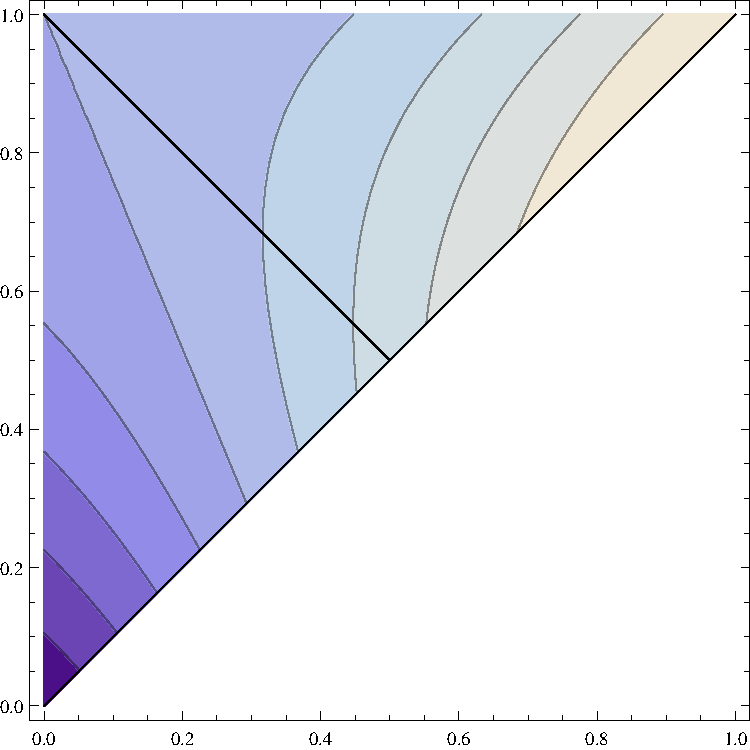
\includegraphics[width = \linewidth]{./plots/welfare.pdf}
\end{minipage} 
\end{figure} 

\subsection{Long-run P2P rental equilibrium} 
In the long-run equilibrium, all parties can revise their ownership decisions. 
The utility from owning is 
\begin{align}
v^{OWN}_i = 2\alpha_i x_i - x_i^2 + (1-x_i)r_{LR} - p   
\end{align} 
whereas the utility from renting is 
\begin{align}
v^{RENT}_{i} = 2\alpha_i x_i - x_i^2 - x_i r_{LR}  
\end{align} 
where $r_{LR}$ is the market-clearing long-run rental rate. 
The first order condition in both choices is $2 \alpha_i - 2 x_i - r_{LR} = 0$ and so $x^* = \alpha_i - r_{LR}/2$. 
Computing the indirect utility for both decisions, we have
\begin{align} 
v^{OWN} = \alpha_i^2 - p + \frac{r_{LR}^2}{4} + (1 - \alpha_i) r_{LR} \quad  \mbox{and} \quad v^{RENT} = \frac{1}{4} (r_{LR}- 2\alpha )^2. 
\end{align} 
Setting $v^{OWN} = v^{RENT}$ to find the conditions under which a user would be indifferent between renting and owning, the $\alpha_i$ term drops out and we are left with 
\begin{align}
p = r_{LR}. 
\end{align}
 \important{In the long-run P2P rental equilibrium, the rental rate equals the product market purchase price and ownership does not depend on usage patterns or valuation.}  

For this new market to clear, we have to determine what fraction of consumers choose to own. 
Let $f$ be the fraction of consumers that purchase the good in equilibrium. 
As ownership does not depend on valuation, we assume that both consumer types are equally likely to own. 
For the market to clear, 
\begin{align}
\left[ (1-x_H(p)) + (1-x_L(p))\right]f = \left(x_H(p) + x_L(p) \right)(1- f) 
\end{align} 
which simplifies to 
\begin{align}
f = \frac{x_H(p) + x_L(p)}{2}.  
\end{align} 
\important{The fraction of consumers owning in the long-run is the average usage rate in the population.}  

In the long-run P2P rental market equilibrium, there are no profits from owning to simply rent-out. 
However, owners and non-owners alike get a surplus. 
\important{This suggests that firms that derive no consumption value from the good can not compete in a competitive: 
because the consumer has excess capacity after satisfying their own consumption, they can ``profitably'' sell their excess capacity at any price and still have positive utility.} 
A firm owning simply to rent would make zero profit. 

\subsection{Product market demand in the long-run P2P rental market equilibrium} 
Most commentators considering the sharing economy have often implicitly assumed that ownership would be reduced under full sharing, the intuition being that there is some fixed amount of demand for some good and that when idle goods are pulled into the market, demand can be met with a smaller total number of goods. 
\important{This is not the case:  
ownership would increase if the product market price was below the rental rate.} 
Intuitively, when the short-run rental rate is creater than the purchase price, a consumer could buy the good at $p$ and rent out the entire capacity for $r$ and since $r > p$, earn a profit. 

To see this algebraically, first consider that in the long-run P2P equilibrium, the new product market demand curve, $D_1$, is
\begin{align}
D_1(p) &= 2f \notag \\  
     &= x_H(p) + x_L(p) \notag \\ 
     &= \alpha_H + \alpha_L - p.  
\end{align} 

In the pre-sharing product market, $D_0(p) = 1$ since all of the high-types purchased the good. 
Let $r_{SR}$ be the short-run rental rate, which we recall from Equation~\ref{eq:strr} is just $\alpha_H + \alpha_L - 1$. 
If demand is higher after the long-run P2P equilibrium emerges, then  
\begin{align} 
D_{1}(p) & > D_{0}(p) \notag \\
\alpha_H + \alpha_L - p &> 1 \notag \\ 
\alpha_H + \alpha_L - 1 &> p \notag \\ 
r_{SR} &>  p. 
\end{align} 

\important{If the market-clearing short-run rental rate is above the purchase price, ownership will increase, otherwise decrease.}
Practically speaking, this is likely to occur in situations where there are high valuations from both consumer types (making demand high and supply tight) as well as relatively low purchase prices, which make ownership more attractive. 

\subsection{Long-run P2P equilibrium product market demand versus the original ``no sharing'' demand} 
Previously, there were ``kinks'' in the product market demand curve at $\alpha_H^2$ and $\alpha_L^2$. 
In the long-run P2P rental equilibrium, product demand now varies continuously, with $D(p) = x_H(p) + x_L(p) = \alpha_H + \alpha_L - p$ when both consumer-types participate. 
Figure~\ref{fig:demand} illustrates the new product market demand curve, with the pre-P2P rental market curve indicated as $D_0$ and the post-P2P rental market by $D_1$. 
One thing to note is that a higher product market price is supportable: the demand curve $D_1$ is non-zero for a range of prices for which $D_0$ is zero.  

% http://tex.stackexchange.com/questions/76418/plot-non-continuous-function-with-tikz
\begin{figure}
\caption{Product market demand pre-P2P rental market and post-P2P rental market (long-run)}
\label{fig:demand} 
\centering
% \begin{tikzpicture}[scale=5]
% \draw (1,0) node[below]{$Q$} -- (0,0) --(0,1) node[left]{$p$};
% \draw[ultra thick] (0,1) to (0, \alphaH^2); 
% \draw (0,\alphaH^2) circle (1pt)
% \end{tikzpicture}
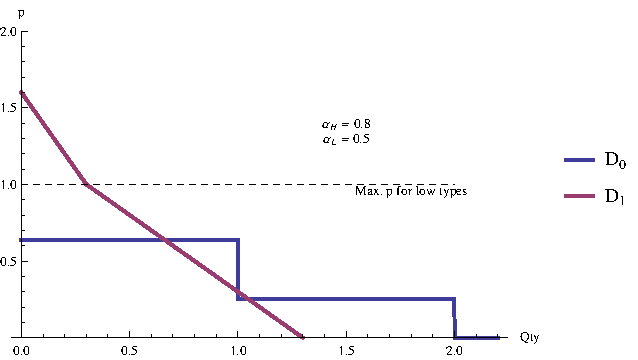
\includegraphics[scale = 1]{./diagrams/p2plr_demand.pdf}
\end{figure} 

Recall that in the pre-P2P rental market with two consumer types, if $p > \alpha_H^2$, then no one bought the good. 
\important{A P2P rental market in long-run equilibrium can support a higher product market price than pre-rental.}  
Intuitively, if a would-be owner can earn rental income from their unused portion, it seems likely that a higher product market price is supportable. 
The highest possible price that can support a market pre-P2P rental is $\bar{p}_0 = \alpha_H^2$.  
In the long-run P2P market, $D(p) = \alpha_H + \alpha_L - p$, and so $\bar{p}_{1} = \alpha_H + \alpha_L$. 
\important{Since $\alpha_H > \alpha_H^2$ and $\alpha_L > 0$, $\bar{p}_1 > \bar{p}_0$: the existence of a P2P rental market can support a higher product market price.} 

The portion of $D_1$ that is non-zero where $D_0$ is not straight---it is actually kinked at $p = 2\alpha_L$. 
\important{The reason for this kink is that if $2\alpha_L < p$, the low-types do not use the good in the long-run P2P equilibrium.} 
The reason is simple: if $p > 2\alpha_L$, usage of the good offers negative utility from any amount of usage and so the low-types use none. 
If $p > 2 \alpha_L$, then the long-run P2P equilibrium is one in which the high-types simply trade with themselves, creating a market demand of just $D(p) = \alpha_H - p/2$. 
\important{The model suggests the possibility of a transitory short-run phase in which low-types get access that disappears once former-owners become renters and bid up rental rates until low-types would get no usage utility at the market rental rate.} 

\subsection{Long-run P2P rental market consumer surplus when both consumer types use the good} 
If both high- and low-types participate in the long-run P2P equilibrium, social surplus is 
\begin{align} 
S_1 & = \frac{1}{4}(p - 2\alpha_H)^2 + \frac{1}{4}(p - 2\alpha_L)^2 \notag \\
    & = \alpha_H^2 + \alpha_L^2 - p(\alpha_H + \alpha_L) + \frac{p^2}{2} \notag \\ 
\end{align} 
whereas in the pre-P2P rental market it was 
\begin{align}
S_0 = \alpha_H^2 - p.  
\end{align} 
The long-run social surplus from the introduction of the P2P rental market is  
\begin{align}
\Delta S = S_1 - S_0 = \alpha_L^2 + (1 - \alpha_L - \alpha_H)p + p^2/2.  
\end{align} 
From the requirement that $\alpha_L^2 < p < \alpha_H^2$ and the assumption that the low-type still consumes some of the good in equilibrium ($2 \alpha_L > p$), we can show that $\Delta S > 0$. 
\important{We can also show that social surplus from the long-run P2P rental market is increasing the low-type valuation, or $\Delta S'(\alpha_L) > 0$, again because $2\alpha_L > p$.}
\important{For the high-types, $\Delta S'(\alpha_H) = -p < 0$, and so the social surplus from sharing is 
reduced when the high-types have a higher valuation.}

\subsection{Transaction costs and depreciation}
Note that in the short-run, $r$ did not depend directly on $p$, but in the long-run they are linked. 
Let $r_{SR}$ be the short-run rental rate and let $r_{LR}$ be the long-run rental rate. 
Let $p_{SR}$ and $p_{LR}$ be the short- and long-run product prices, respectively.  

If $r_{SR} > p_{SR} + \gamma$, there were excess profits available to being an owner. 
As such, in the long-run, demand in the product market will go up, raising $p_{LR}$ and lowering $r_{SR}$. 
In this case, the emergence of the sharing economy causes a Jevon's paradox of increased usage. 
Producer surplus rises, but the effect on consumers is ambiguous. 
Long-run non-sharers are made strictly worse-off, as they now face a higher price in the product market. 
All consumers that would not have purchased under the pre-sharing regime are better off, as they consumer some of the good.

On the contrary, if $r_{SR} < p_{SR} + \gamma$, ownership is less attractive and in the long-run, fewer goods will be purchased, lowering prices. 
In this case, the introduction of the sharing economy is Pareto improving with respect to consumers. 
Owners that do not rent out their good get a price reduction; former non-owners get to consume some of the good. 
For owners that rent out the good, they could consumer their old $x$ (pre-sharing) at a now-lower purchase price and so are strictly better off. 

Many goods have ``missing'' rental markets despite generating usage far below $x = 1$ because the rental rate $r$ required to cover the added transaction costs of renting would be too high to create a viable rental market. 

Suppose it costs the firm $\gamma$ to full rent-out an owned product and suppose rental goods have to be purchased in the product market. 
No arbitrage would mean that $p + \gamma = r$. 

\section{The attributes of goods and the feasibility of renting} 

The model deliberately abstracts away from the nature of the good being transacted, but presumably some attributes of the good determine how ``rentable''  or ``shareable'' it actually is. 
If we look to what is currently commonly rented, we get some sense of what makes something amenable to renting:  
goods that are used infrequently but are expensive and/or are difficult to transport: 
cars and hotels in distant cities, tuxedos, certain kinds of specialty tools (e.g., rototillers, carpet shampoers) and so on. 

As discussed earlier, it is only with the emergence of computer-mediate platforms that seem to dramatically reduce transaction costs that a P2P rental market has emerged for some of these goods. 
Before these markets sprung up, simply finding an appropriate trading partner would be difficult, to say nothing of coming to terms, writing a contract, monitoring compliance, handling disputes, making payment and so on. 
If transaction costs were sufficiently high, then the rental rate would be too high to support a market (even though the high rental rate would tend to stimulate supply). 

The model predicts that goods with high purchase prices but low per-consumer usage are ideal for P2P rental markets in the short-run: 
the purchase price is high enough that there are lots of would-be consumers with high willingness to pay and enough owners with excess capacity that the market-clearing rental rate is not prohibitively high. 
When produce market prices are low, there is no excess demand so nearly everyone buys the product, so even if the good is used infrequently, no rental market can exist.  
For example, there is no rental market in kitchen timers---although they are used infrequently and quite durable, there is neither supply (no one owning finds it worth the trouble to rent them out) nor demand (if one wants one, they go to the product market). 
Other goods are expensive but there is no excess capacity, as they are used more or less continuously. 
For example, there is and can be no P2P rental market in dentures. 
Other goods are used infrequently and are expensive but make poor sharing candidates because demand is so unpredictable. 
For example, a gas-powered back-up electrical generator is used infrequently but would be difficult to rent in a P2P market, as demand is likely to be correlated in space and time. 

Goods that are difficult to transport but need to be used in a different locations will be hard to rent. 
However, goods that can be used on-site by different people are more shareable. 
For example, yachts are relatively difficult to transport long distances, but there is a thriving P2P rental market in boats where many want to sail on vacation: 
in the British Virgin islands charter yachts are owned by individuals. 

Nearly all goods, even if classified as ``durable'' do get used up through consumption. 
Depreciation can partially be offset through careful use and monitoring as well as maintenance.  
Most things---apartments, cars, clothes etc., need to be cleaned and or serviced before they can be rented again. 
However, other goods like jewelry presumably have little ``reset'' cost.

In the model, if a good is used $x$, $1-x$ is available to rent, with would-be renters indifferent over which ``piece'' of the $1$ unit they get. 
Several practical considerations might this assumption problematic. 
The usage of some goods cannot be cleanly divided into large chunks of time: 
some goods, even if used rarely in total, are used intermittently. 
For example, a fly-swatter generally is not used very often (giving lots of $1-x$), but when it will be used is highly unpredictable. 
Other goods can be nicely divided: it is easy for one family to use a vacation home one week while another family uses it another week. 
Goods with predictable or easily adjustable usage patterns are more likely to be P2P rental. 

\subsection{Design and administration of the survey}

Using Amazon Mechanical Turk, I hired US-based workers to answer a questions about a consumer good, e.g., BBQ grill, pick-up truck, men's suit, toothbrush etc.
I asked them: whether they owned the good; whether they had ever rented or lent out the good; how much they would use the good \emph{regardless} of whether they actually owned the good; their reasons for not owning the good; whether they would use the good in one large chunk or many small chunks; whether usage was predictable; why they did not own the good; and finally, what was their household income. 
See Appendix~\ref{sec:survey} for the full list of goods as well as the actual survey questions and answers.  
Each ``human intelligence task'' or HIT was about one particular good. 
Workers were allowed to answer for each of the 20 goods.  

The MTurk is a convenience sample, but there is no strong reason to think they would have highly idiosyncratic consumption patterns. 

but it has been used effectively by other researchers in a variety of settings. 
For example, \cite{kuziemko2013elastic} uses it to elicit TK. 

\subsection{Ownership and renting patterns} 

Figure~\ref{fig:frac_owning} shows the fraction of respondents reporting owning various goods.  
There are few surprises: nearly everyone owns a toothbrush, a hammer and a blender; no one reported owning a jet ski and only one reported owning a vacation home.
Figure~\ref{fig:frac_renting} shows the fraction of respondents reporting having rented the various goods. 
Generally, ownership and renting appear to be gross substitutes, with the notable exception of cars (presumably because people rent cars when traveling). 

\begin{figure}
\centering 
\caption{Fraction of respondents owning various goods \label{fig:frac_owning} }
\begin{minipage}{0.90 \linewidth}
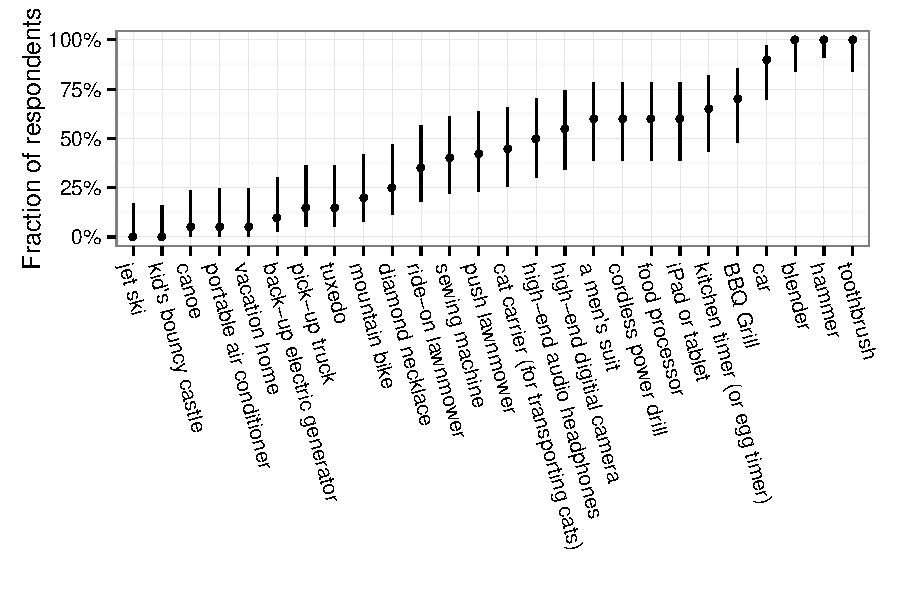
\includegraphics[width = \linewidth]{./plots/ownership_fractions.pdf} 
\end{minipage} 
\end{figure} 

\begin{figure}
\centering 
\caption{Fraction of respondents reporting having rented various goods \label{fig:frac_renting}}
\begin{minipage}{0.90 \linewidth}
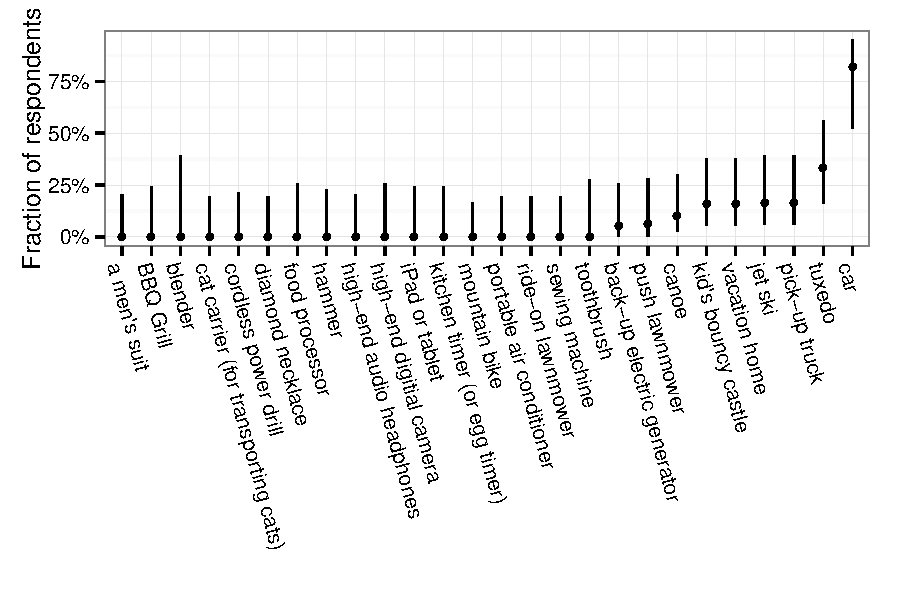
\includegraphics[width = \linewidth]{./plots/rental_fractions.pdf} 
\end{minipage} 
\end{figure} 

Figure~\ref{fig:scatter} plots the fraction of respondents reporting having rented a good versus the fraction owning, on a square-root scale.  
There is generally a negative relationship between owning and renting. 
Goods that are used during special occasions like weddings, celebrations and vacations show the highest rates of rental and lowest rates of ownership, e.g., tuxedos, vacation homes, jet ski, tuxedos, canoe's, bouncy castles. 
There may also be some evidence of expensive tools useful for one-off jobs being rented, such as an electric generator and a pick-up truck. 
Unsurprisingly, goods with nearly universal ownership show little renting with the notable exception of cars, which are both owned and rented at high rates, presumably because people rent cars when traveling.  
\important{There are a number of goods (not all labeled) that show medium ownership levels (e.g., around 50\%) and yet zero recorded instances of renting.} 

To confirm the visual pattern of renting declining in ownership, I report the results of two OLS regressions of the form
\begin{align}
\mbox{FracRent} = \beta_0 + \beta_1 \mbox{FracOwn} + \epsilon,  
\end{align} 
where $\mbox{FracOwn}$ is the fraction of respondents claiming to own the good and $\mbox{FracRent}$ as the faction claiming to have rented the good. 
Table~\ref{tab:own_vs_rent} reports the estimated regression of this equation, with cars included in Column~(1) and cars excluded in Column~(2). 
We can clearly see the importance of cars in the overall pattern: while both regression estimates have a negative slope, the effects are much stronger when cars are excluded. 

\begin{figure}
\centering 
\caption{Fraction renting versus fraction owning \label{fig:scatter} }
\begin{minipage}{0.60 \linewidth}
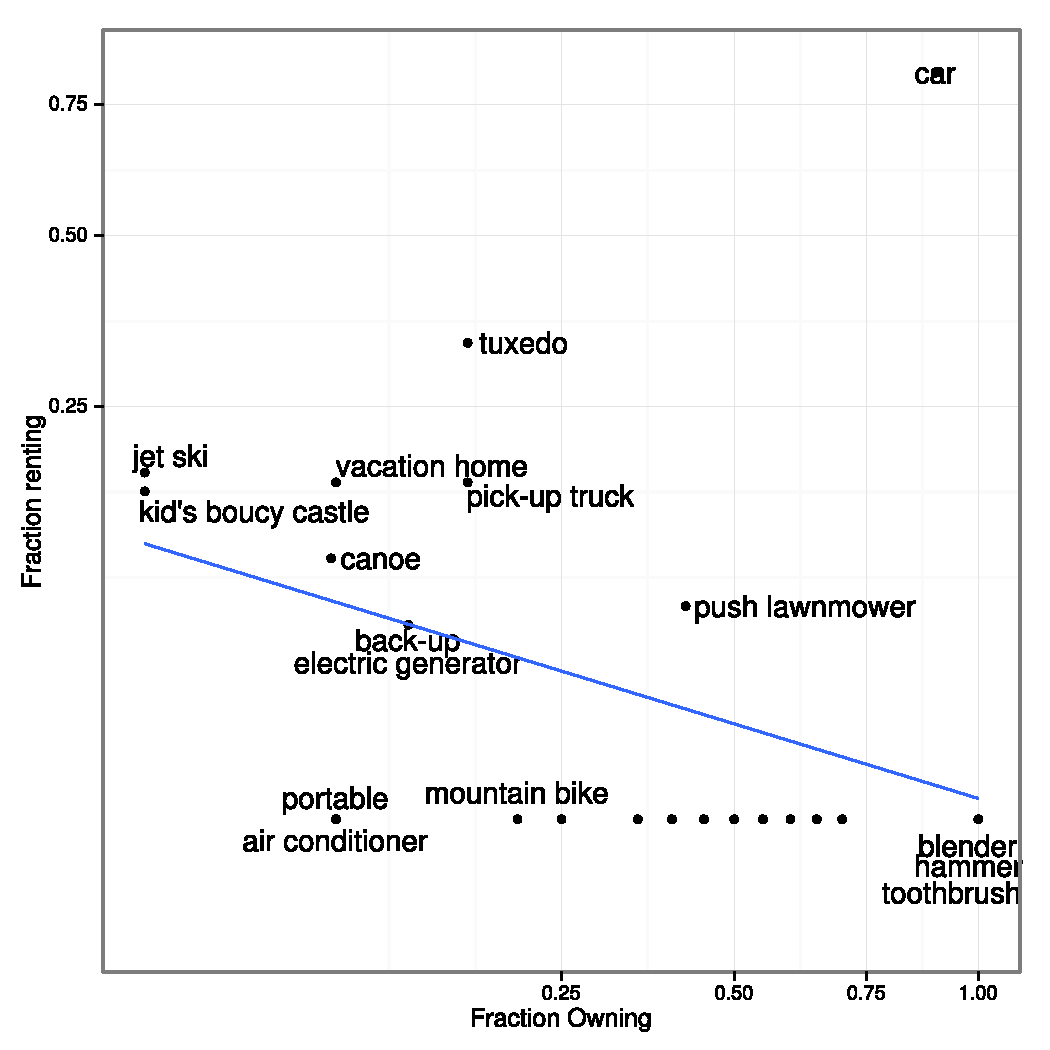
\includegraphics[width = \linewidth]{./plots/scatter_rent_v_own.pdf} 
\end{minipage} 
\end{figure} 


% Table created by stargazer v.5.2 by Marek Hlavac, Harvard University. E-mail: hlavac at fas.harvard.edu
% Date and time: Tue, Jan 26, 2016 - 07:25:21 AM
% Requires LaTeX packages: dcolumn 
\begin{table}[!htbp] \centering 
  \caption{Fraction of respondents owning a good versus fraction having rented a good} 
  \label{tab:own_vs_rent} 
\footnotesize 
\begin{tabular}{@{\extracolsep{5pt}}lD{.}{.}{-3} D{.}{.}{-3} } 
\\[-1.8ex]\hline 
\hline \\[-1.8ex] 
 & \multicolumn{2}{c}{\textit{Dependent variable:}} \\ 
\cline{2-3} 
\\[-1.8ex] & \multicolumn{2}{c}{Fraction reporting renting the good (\textsc{FracRental})} \\ 
\\[-1.8ex] & \multicolumn{1}{c}{(1)} & \multicolumn{1}{c}{(2)}\\ 
\hline \\[-1.8ex] 
 Fraction reporting owning the good & -0.009 & -0.160^{***} \\ 
  & (0.109) & (0.046) \\ 
  Constant & 0.081 & 0.115^{***} \\ 
  & (0.059) & (0.024) \\ 
 \hline \\[-1.8ex] 
Sample & \multicolumn{1}{c}{All Goods} & \multicolumn{1}{c}{Cars Excluded} \\ 
Observations & \multicolumn{1}{c}{26} & \multicolumn{1}{c}{25} \\ 
R$^{2}$ & \multicolumn{1}{c}{0.0003} & \multicolumn{1}{c}{0.345} \\ 
\hline 
\hline \\[-1.8ex] 
\end{tabular}
\\{\footnotesize \begin{minipage}{0.85 \linewidth} \emph{Notes:}
The unit of observation for the regressions in this table is the individual good.
The dependent variable is the fraction of respondents reporting having rented that good, while the independent variable is the fraction reporting owning that good. 
Column~(1) includes all goods surveyed, while Column~(2) excludes cars.
For the full list of goods and the survey language, see Appendix~\ref{sec:survey}. 
\starlanguage \end{minipage} }
\end{table}


\subsection{Lending} 
Even in the absence of P2P rental markets, individuals can still lend goods to each other. 
Figure~\ref{fig:lending} shows the fraction of owners reporting having lent an item to someone else.  

Goods that had the highest fraction of individuals reporting renting are not frequently lent out. 
This is not surprising, as they are not widely owned: 
no one lends out bouncy castles, jet skis, canoes, vacation homes etc. because almost no one in the sampled owns them. 
Further, goods that are nearly universally owned in the sample are not very likely to be lent out: 
for example, blenders are infrequently lent out despite being owned by all respondents---but there presumably is not much demand since this ``owned by everyone'' is generally true in the population. 
The ``sweet spot'' for lending appears to be goods with middling rates of ownership:  


\begin{figure}
\centering 
\caption{Fraction of respondents reporting having lent-out various goods \label{fig:lending}}
\begin{minipage}{0.90 \linewidth}
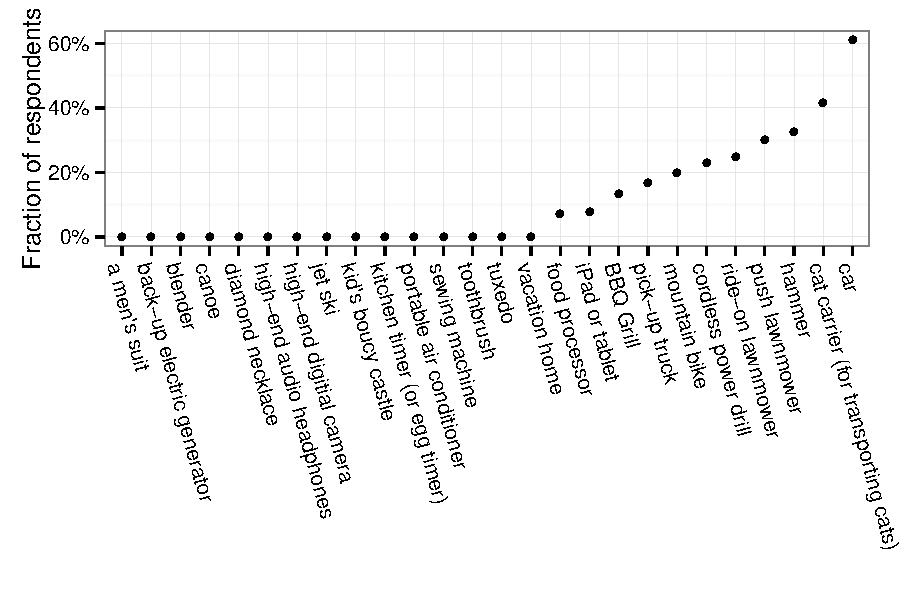
\includegraphics[width = \linewidth]{./plots/lent_fractions.pdf} 
\end{minipage} 
\end{figure} 

Figure~\ref{fig:scatter_lending} shows the scatter plot of fraction of respondents lending out a good versus the fraction owning a good. 

\begin{figure}
\centering 
\caption{Fraction lending versus fraction owning \label{fig:scatter_lending} }
\begin{minipage}{0.60 \linewidth}
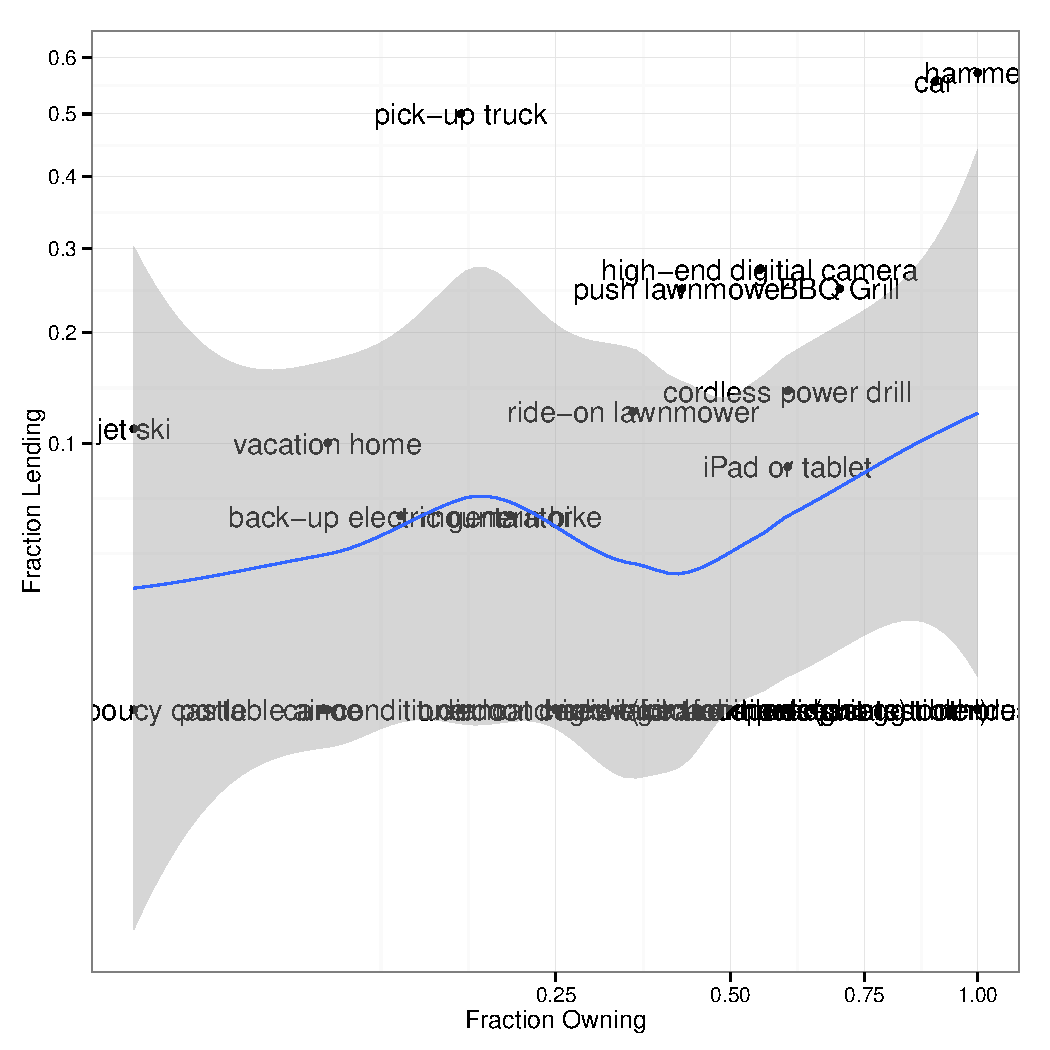
\includegraphics[width = \linewidth]{./plots/lent_v_own.pdf} 
\end{minipage} 
\end{figure} 


\subsection{Predictability and granularity of usage by good} 

Figure~\ref{fig:predict_index} shows the mean prediction index per good. 
Figure~\ref{fig:granularity} shows the mean granularity index per good. 

\begin{figure}
\centering 
\caption{Mean predictability index \label{fig:predict_index} }
\begin{minipage}{0.90 \linewidth}
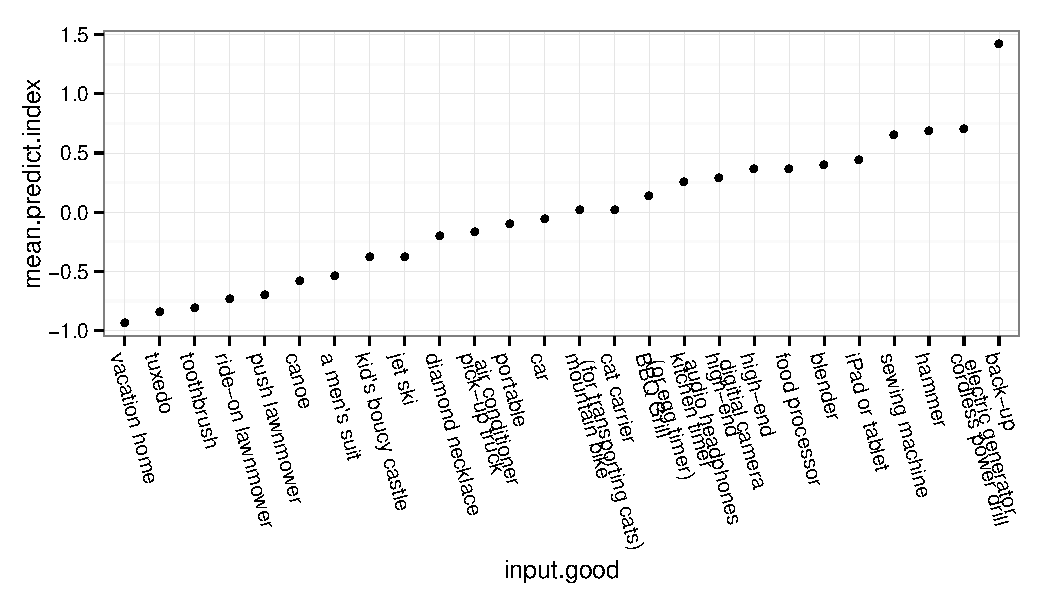
\includegraphics[width = \linewidth]{./plots/predictability.pdf} 
\end{minipage} 
\end{figure} 

\begin{figure}
\centering 
\caption{Mean granularity index \label{fig:granularity}}
\begin{minipage}{0.90 \linewidth}
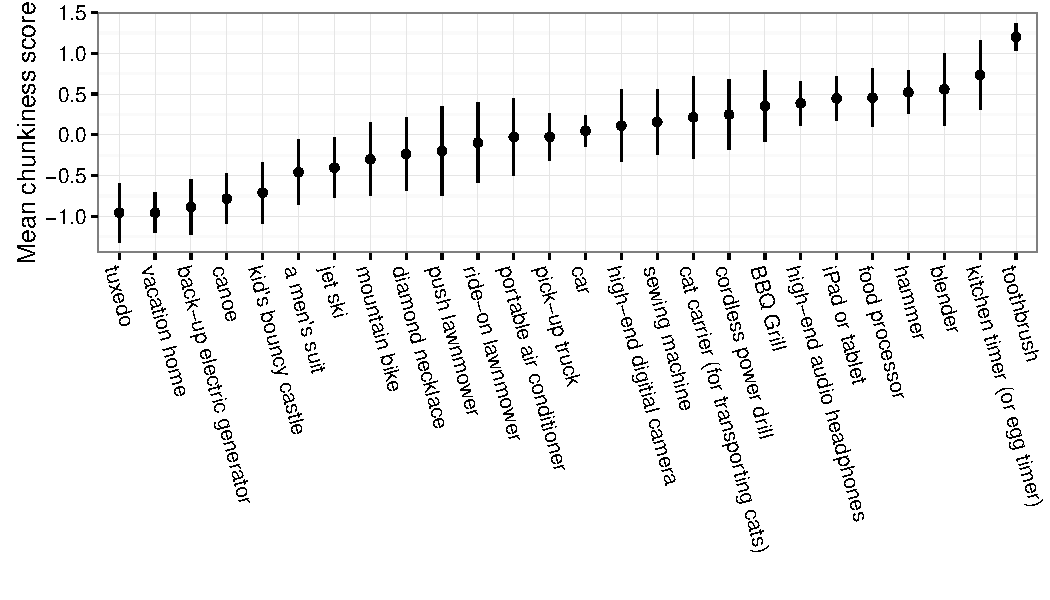
\includegraphics[width = \linewidth]{./plots/granularity.pdf} 
\end{minipage} 
\end{figure} 

\subsection{Ownership and income}

Figure~\ref{fig:ownership_fractions_income} shows the fraction owning various goods by income level.  

\begin{figure}
\centering 
\caption{Variation in ownership by income \label{fig:ownership_fractions_income}}
\begin{minipage}{0.90 \linewidth}
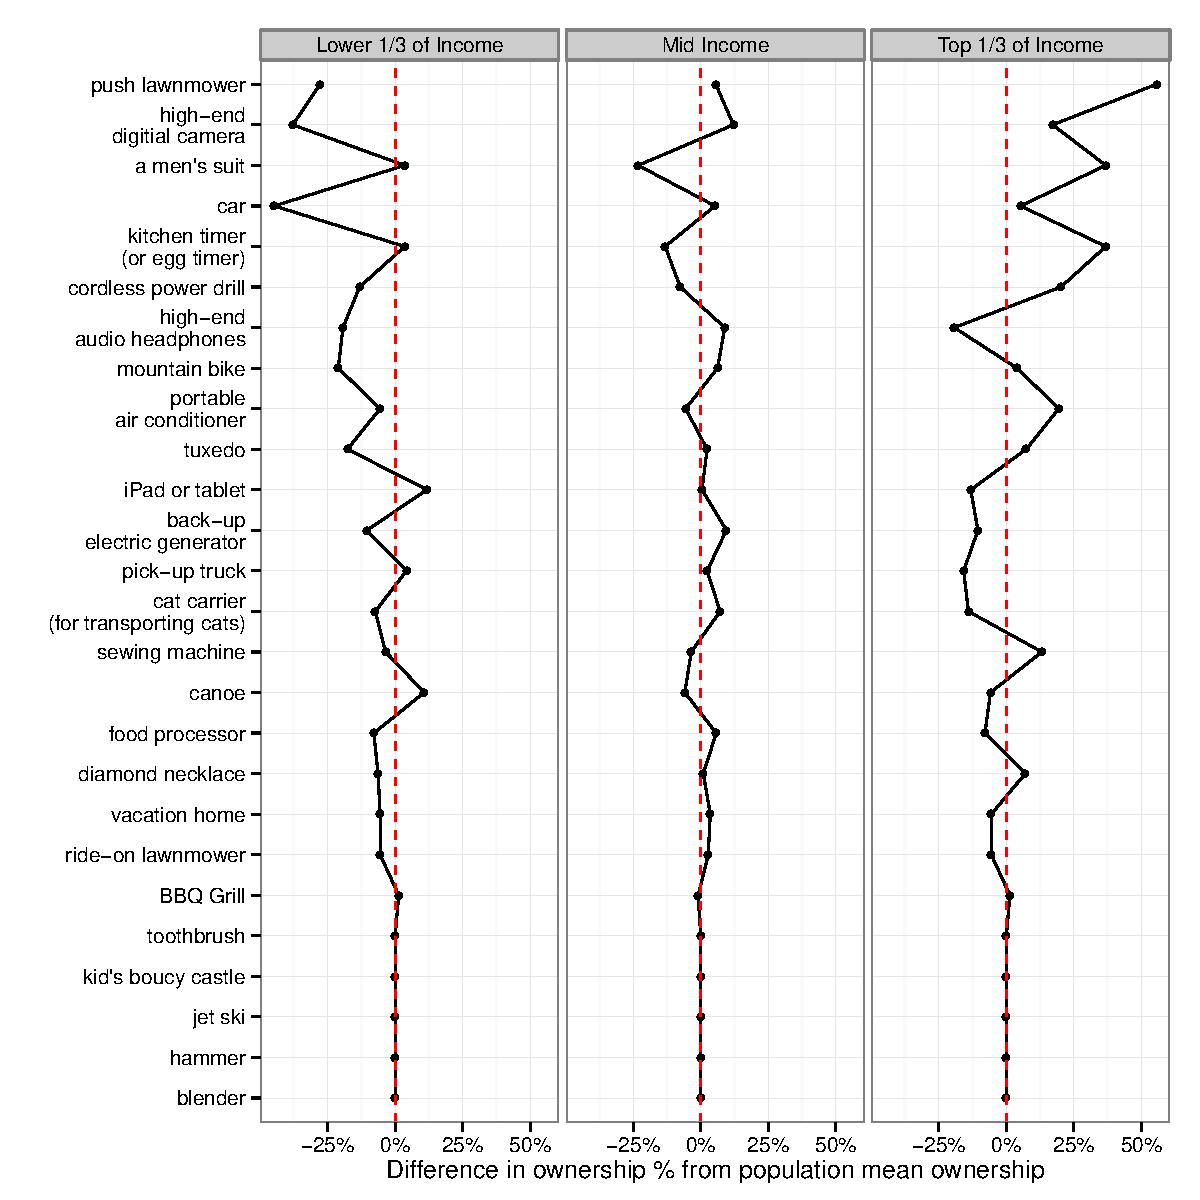
\includegraphics[width = \linewidth]{./plots/ownership_fractions_inc.pdf} 
\end{minipage} 
\end{figure} 

\subsection{Ownership and usage} 

Table~\ref{tab:ownership} shows that TK. 


% Table created by stargazer v.5.1 by Marek Hlavac, Harvard University. E-mail: hlavac at fas.harvard.edu
% Date and time: Thu, May 14, 2015 - 07:55:45 AM
% Requires LaTeX packages: dcolumn 
\begin{table}[!htbp] \centering 
  \caption{Respondent estimates of the fraction of time spent using a good and whether they own that good} 
  \label{tab:ownership} 
\footnotesize 
\begin{tabular}{@{\extracolsep{5pt}}lD{.}{.}{-3} D{.}{.}{-3} D{.}{.}{-3} } 
\\[-1.8ex]\hline 
\hline \\[-1.8ex] 
 & \multicolumn{3}{c}{\textit{Dependent variable:}} \\ 
\cline{2-4} 
\\[-1.8ex] & \multicolumn{3}{c}{Respondent owns the item?, ($\textsc{Own}_{ig}=1$)} \\ 
\\[-1.8ex] & \multicolumn{1}{c}{(1)} & \multicolumn{1}{c}{(2)} & \multicolumn{1}{c}{(3)}\\ 
\hline \\[-1.8ex] 
 Log estimated usage, $\log x_{ig}$ & 0.026^{**} & 0.026^{**} & 0.026^{**} \\ 
  & (0.011) & (0.011) & (0.011) \\ 
  Log household income, $\log y_i$ &  & 0.102^{***} &  \\ 
  &  & (0.025) &  \\ 
 \hline \\[-1.8ex] 
Good FE & \multicolumn{1}{c}{Y} & \multicolumn{1}{c}{Y} & \multicolumn{1}{c}{Y} \\ 
Respondent FE & \multicolumn{1}{c}{N} & \multicolumn{1}{c}{N} & \multicolumn{1}{c}{Y} \\ 
Observations & \multicolumn{1}{c}{411} & \multicolumn{1}{c}{411} & \multicolumn{1}{c}{411} \\ 
R$^{2}$ & \multicolumn{1}{c}{0.445} & \multicolumn{1}{c}{0.465} & \multicolumn{1}{c}{0.567} \\ 
\hline 
\hline \\[-1.8ex] 
\end{tabular}
\\{\footnotesize \begin{minipage}{0.75 \linewidth} \emph{Notes:}
This table reports OLS regressions where the dependent variable is an indicator for whether a respondent reported owning a particular good.
In Column~(1) the independent variable is that respondent's estimate of what fraction of their time they would spend using that good (in logs).
In Column~(2) a regressor for the log of the respondent's self-reported household income is added to the Column~(1) specification.
Column~(3) uses the same specification as Column~(1), but a respondent specific fixed effect is added. 
The sample is restricted to respondents who reports some positive amount of predicted usage of the good and reported their household income.
All regressions include good-specific fixed effects and standard errors are clustered at the good level. 
\starlanguage \end{minipage} }
\end{table}


Table~\ref{tab:ownership_attr} explores how the perceived usage attributes of the good are related to the ownership decision.
My hypothesis was that goods with an unpredictable usage pattern and/or whose usage was spread out over many small chunks would necessitate ownership. 
In Column~(1), we see that the less predictable perceived usage, the more likely the good is to be owned. 
In Column~(2), the more granular usage is, the more likely the good it to be owned. 


% Table created by stargazer v.5.2 by Marek Hlavac, Harvard University. E-mail: hlavac at fas.harvard.edu
% Date and time: Tue, Jan 26, 2016 - 07:25:30 AM
% Requires LaTeX packages: dcolumn 
\begin{table}[!htbp] \centering 
  \caption{Good usage unpredictability and chunkiness and its association with good ownership.} 
  \label{tab:ownership_attr} 
\footnotesize 
\begin{tabular}{@{\extracolsep{5pt}}lD{.}{.}{-3} D{.}{.}{-3} D{.}{.}{-3} D{.}{.}{-3} } 
\\[-1.8ex]\hline 
\hline \\[-1.8ex] 
 & \multicolumn{4}{c}{\textit{Dependent variable:}} \\ 
\cline{2-5} 
\\[-1.8ex] & \multicolumn{4}{c}{Item is owned} \\ 
\\[-1.8ex] & \multicolumn{1}{c}{(1)} & \multicolumn{1}{c}{(2)} & \multicolumn{1}{c}{(3)} & \multicolumn{1}{c}{(4)}\\ 
\hline \\[-1.8ex] 
 Unpredictability Score (US) & 0.139^{***} &  & 0.095^{***} & 0.003 \\ 
  & (0.030) &  & (0.034) & (0.034) \\ 
  Chunkiness Score (CS) &  & 0.135^{***} & 0.091^{***} & -0.018 \\ 
  &  & (0.025) & (0.029) & (0.025) \\ 
  US x CS &  &  & -0.009 & 0.006 \\ 
  &  &  & (0.018) & (0.018) \\ 
 \hline \\[-1.8ex] 
Respondent FE & \multicolumn{1}{c}{Y} & \multicolumn{1}{c}{Y} & \multicolumn{1}{c}{Y} & \multicolumn{1}{c}{Y} \\ 
Good FE & \multicolumn{1}{c}{N} & \multicolumn{1}{c}{N} & \multicolumn{1}{c}{N} & \multicolumn{1}{c}{Y} \\ 
Observations & \multicolumn{1}{c}{489} & \multicolumn{1}{c}{489} & \multicolumn{1}{c}{489} & \multicolumn{1}{c}{489} \\ 
R$^{2}$ & \multicolumn{1}{c}{0.170} & \multicolumn{1}{c}{0.169} & \multicolumn{1}{c}{0.191} & \multicolumn{1}{c}{0.500} \\ 
\hline 
\hline \\[-1.8ex] 
\end{tabular}
\\ {\footnotesize  \begin{minipage}{0.85 \linewidth} \emph{Notes:}
This table reports regressions of an indicator for whether the respondent owns a good on that same respondent's estimates of the unpredictability and granularity of usage for that good.
The two indices are normalized responses to the 1-5 scale questions on usage chunkiness and unpredictability, pooled over all respondents and goods.
Toothbrushes and backup generators are excluded from the sample. 
See Appendix~\ref{sec:survey} for the actual survey language and responses.
In each regression, a respondent-specific fixed effect is included.
Standard errors are clustered at the level of the individual respondent.
\starlanguage
\end{minipage} }
\end{table}
 

In this model presented in this paper, preferences are still primitives of the model, but they are modeled as differences in planned \emph{usage} of the good.  

Figure~\ref{fig:usage_by_own} the boxplot distributions of reported usage by ownership. 

\begin{figure}
\centering 
\caption{Distribution of usage indexes by ownership}
\label{fig:usage_by_own}
\begin{minipage}{0.90 \linewidth}
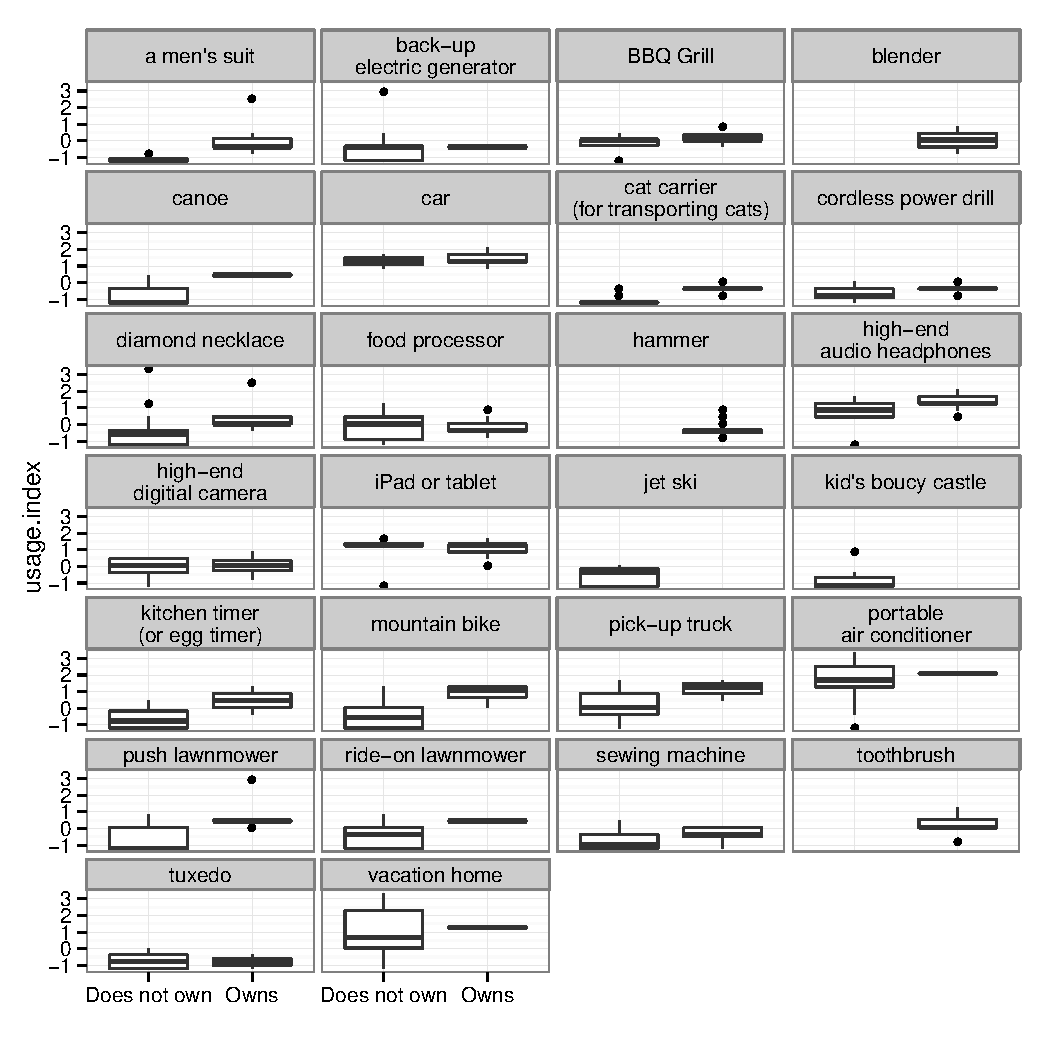
\includegraphics[width = \linewidth]{./plots/usage_by_own.pdf} 
\\
{\footnotesize
\emph{Notes:} Here are some notes. 
}
\end{minipage} 
\end{figure} 

\subsection{Lending and attributes}

\subsection{Reasons for non-ownership} 

Figure~\ref{fig:reasons} are the reasons for not owning, per good. 

\begin{figure}
\centering 
\caption{Reasons given for non-ownership} 
\label{fig:reasons}
\begin{minipage}{0.90 \linewidth}
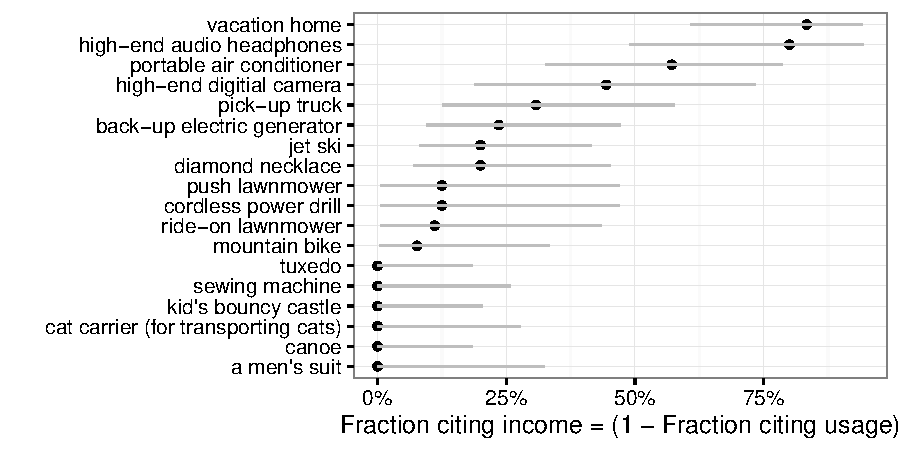
\includegraphics[width = \linewidth]{./plots/reasons.pdf} 
\end{minipage} 
\end{figure} 


\begin{figure}
\centering 
\caption{Ownership fractions by family income quartiles}
\begin{minipage}{0.90 \linewidth}
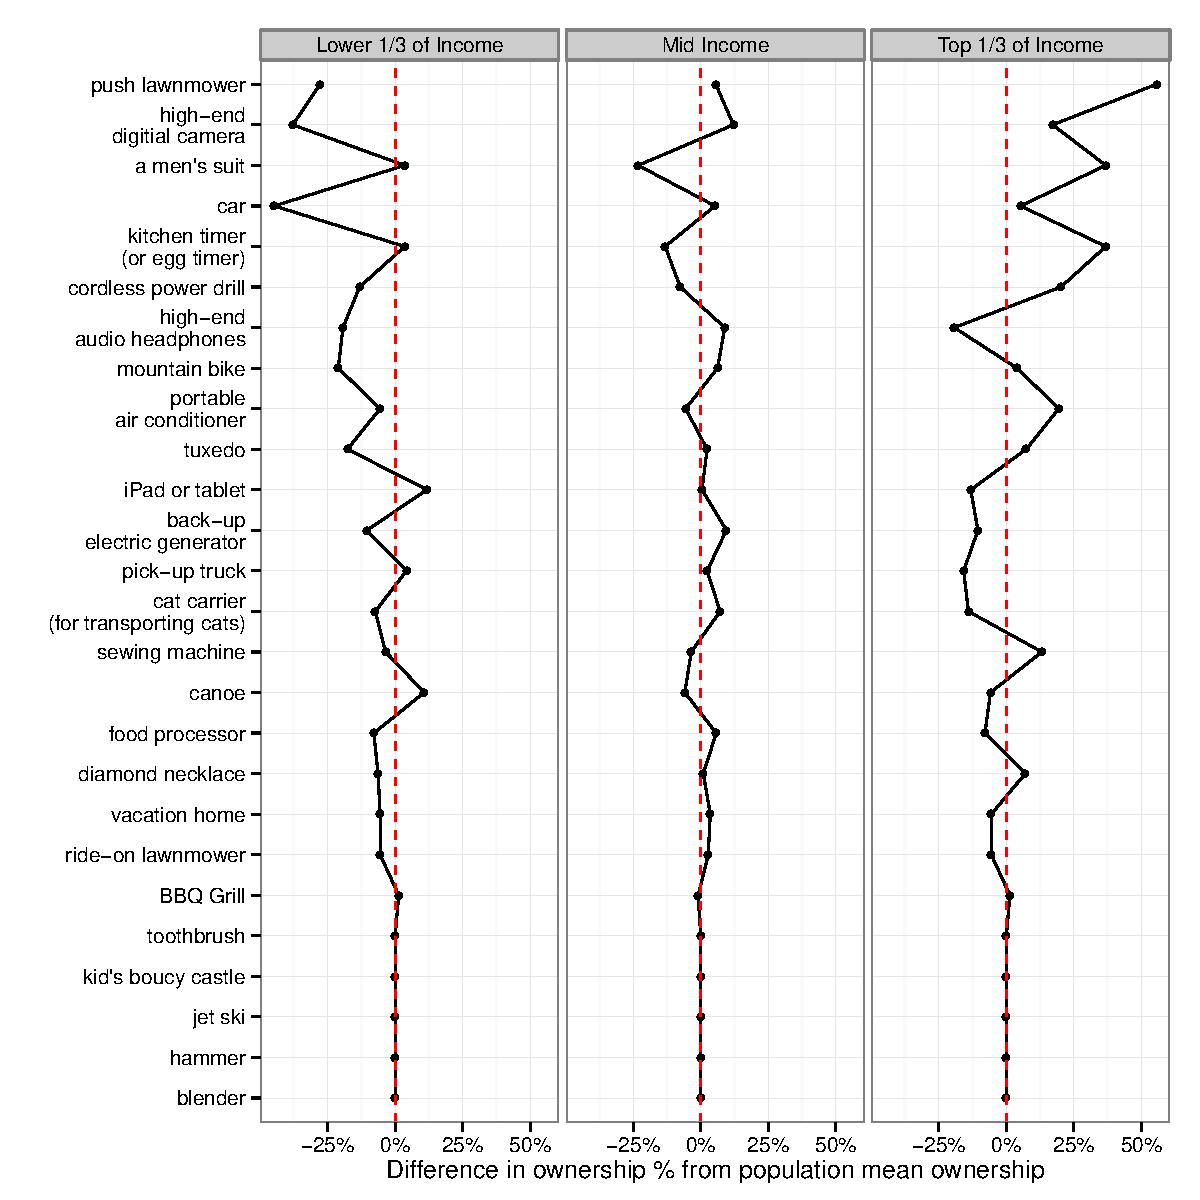
\includegraphics[width = \linewidth]{./plots/ownership_fractions_inc.pdf} 
\end{minipage} 
\end{figure} 

\section{Discussion} 
 
\subsection{Taste for diversity} 
In some formulations of the consumer problem, consumers consume some positive amount of every good offered.
For example, a Cobb-Douglas utility function has no corner solutions---every good is consumed at least a little bit.
This is obviously a large departure from empirical reality if we draw find-grained distinctions between ``goods.'' 
For example, Amazon.com currently lists 6,238 results for "blender" in the Home \& Kitchen category: 
presumably most households own far fewer than this, with most owning 1 or 0.
The reason for this pattern in the language of this model is clear: 
a consumer's $\alpha$ for Blender 2 \emph{conditional} upon owning Blender 1 is quite low and so another blender is not purchased.   
There are numerous goods that have highly negative cross price elasticities but that would not in a world of perfectly competitive rental markets in all goods.  
Very few people rent the same car they drive or vacation in their home towns. 
   

Goods that have a high novelty value are particularly amenable to renting: 
This explains why rentals or lending of videos and books are/were commonplace.  

\subsection{Product market changes to facilitate rentals} 

\section{Conclusion}
In the very long-run, product differentiation could move towards making sharing more attractive. 
Individuals will purchase more durable goods to reduce the frequency of replacement. 
Goods with broad appeal will see an increase in demand compared to more idiosyncratic goods that cater to the owner's taste (similar to how re-sale value enters into some consumers decisions now). 
There will be a shift towards products that are more easily shareable. 
For example, locks on cars and houses that allow remote entry will be more appealing. 

On-going technological developments should reduce the costs of sharing. 
The Internet-of-Things will make it easier to identify goods that are not being used at a moment in time. 
It will also permit more instrumentation which in turn should facilitate contracting. 
For example, many goods might make a high resolution video, with precise time-tracked location of how they are being used, reducing concerns about moral hazard. 
As more of economic and social life are computer-mediated, platforms will use this information to verify the identify and reputation of buyers and sellers, mitigating moral hazard and adverse selection.  

Product market producers will subsidize sharing of experience goods, say by offering them at a discount to known-sharers.\footnote{GM is already doing this with RelayRides}.  

For goods for which Jevon's paradox does not hold, marketing will be re-directed towards encouraging ownership.
Barring that, advertisers will trumpet the rental stream income from a purchase and highlight the advantages of residual control rights. 
We might see more B2B rentals, particular among companies that have similar inputs but are not competitors in the product market. 
Goods with declining real prices are unattractive for sharing businesses, as the trend will be towards ownership. 

Digital goods are incredibly attractive for P2P ``rental'' but since a single owner can meet all the demand among non-owners, the rental rate is zero.
The reason is that even if the owner uses $x$, $1$ is still available to the person ``rented'' to.  
Of course, this is just piracy. 

%IP-multiplexing 

\cite{sinai2005}
\cite{ikkala2014defining}
\cite{varian2000} 
\cite{byers2013rise} 
\cite{becker1965theory} 

\bibliographystyle{aer}
\bibliography{sharing.bib}

\newpage 

\appendix 

\section{Survey Questions \label{sec:survey}} 

The actual goods were: 

\begin{itemize} 
\item BBQ Grill
\item toothbrush
\item a men's suit
\item blender
\item canoe
\item car
\item cordless power drill
\item hammer
\item diamond necklace
\item food processor
\item hammer
\item cat carrier (for transporting cats)
\item high-end audio headphones
\item high-end digitial [sic] camera
\item iPad or tablet
\item jet ski
\item kid's boucy [sic] castle
\item kitchen timer (or egg timer)
\item mountain bike
\item pick-up truck
\item push lawnmower
\item ride-on lawnmower
\item tuxedo
\item vacation home
\item back-up electric generator
\item portable air conditioner
\item sewing machine
\end{itemize} 

\begin{itemize} 

\item Does your household own a {\bf good}?
\begin{itemize}
\item Yes
\item No
\end{itemize} 

\item Have you ever lent your {\bf good} to someone else?
\begin{itemize}
\item Yes
\item No
\item NA - we do not own one.
\end{itemize} 

\item Have you ever borrowed a {\bf good} from someone else?
\begin{itemize}
\item Yes
\item No
\item NA - we own one.
\end{itemize} 

\item Have you ever rented a {\bf good}?
\begin{itemize}
\item Yes
\item No
\item NA - we own one.
\end{itemize} 

\item Regardless of whether your household owns a {\bf good}, if you did own one, how much do you estimate it would be used by members of your household on average?

\begin{itemize} 
\item We would not use this at all
\item 1 minute a week (about 1 hour a year) 
\item 5 minutes a week (about 4 hours a year)
\item 1/2 an hour a week
\item 1 hour a week
\item 1/2 an hour a day
\item 1 hour a day
\item 2 hours a day
\item 4 hours a day
\item 8 hours a day
\item 16 hours a day
\item 24 hours a day (I would continuously be using this good)
\end{itemize} 


\item Regardless of whether you actually own a {\bf good}, how do you imagine it would be used if it was owned by your household (on a scale of 1 to 5): 
\begin{itemize} 
\item 1 - Used in one big block of time
\item 2  
\item 3 - Used in a mixture of large and small blocks of time
\item 4 
\item 5 - Used in many small blocks of time
\end{itemize} 

\item Regardless of whether you actually own a {\bf good}, how predictable would your usage of it be if you did own it: 
\begin{itemize}
\item 1 - Very predictable---I can plan usage many weeks in advance
\item 2  
\item 3 - Somewhat predictable 
\item 4 
\item 5 - Very unpredictable---I would never know exactly when I would need to use it until right beforehand. 
\end{itemize} 

\item If you do not own a {\bf good}, what is the primary reason?
\begin{itemize} 
\item NA - we own one.
\item We wouldn't use it enough to justify the purchase price
\item We would use it, but we simply do not have the money.
\item I don't have the space for this item
\end{itemize} 

\item What is your total household income? 
\begin{itemize} 
\item Less than \$10,000
\item  \$10,000-\$19,999
\item  \$20,000-\$29,999
\item  \$30,000-\$39,999
\item  \$40,000-\$49,999
\item  \$50,000-\$59,999
\item  \$60,000-\$69,999
\item  \$70,000-\$79,999
\item  \$80,000-\$89,999
\item  \$90,000-\$99,999
\item  \$100,000-\$149,000
\item  More than \$150,000
\end{itemize} 

\end{itemize}

\end{document} 

